\documentclass[a4paper,11pt]{article}
\usepackage[utf8]{inputenc}
\usepackage[T1]{fontenc}
\usepackage[a4paper]{geometry}
\geometry{top=2.54cm, bottom=2.54cm, left=2.54cm, right=2.54cm}
\usepackage[spanish]{babel}
\usepackage{amssymb, amsmath}
\usepackage{graphicx}
\graphicspath{ {RepoProyecto/} }
\usepackage{caption}
\usepackage{float}
\usepackage{subcaption}
\usepackage{hyperref}

\title{Microplásticos en Agua Potable}
\author{Aniel Fumero Hernández}
\begin{document}

\maketitle
	\begin{abstract}
	
	URL del repositorio en GitHub:  \href{https://github.com/Drakke4239/proyecto\_final}{https://github.com/Drakke4239/proyecto\_final}.\\
	\\Este estudio investiga el contenido de partículas de microplásticos (MPs) en agua limpia y sobre todo en agua potable. Especificamente, de 3 plantas de tratamiento de agua (WTPs). Encontrandose en todas ellas la presencia de MPs de tamaño de partícula variable.\\\\
	\textbf{Palabras claves:} Agua potable, Plantas de tratamiento de agua, Microplásticos.
	
	\end{abstract}
\tableofcontents
\section{Introducción}
En este estudio se hace uso de muestras de agua tratadas y sin tratar de plantas de tratamiento de agua(WTPs). Todas ellas utilizan sistemas diferentes en el tratamiento y la fuente de agua que toman, así se evitan errores. Por la misma razón se tomaron las muestras en invierno, minimizando la variación de los resultados por interferencias con fitoplacton.
Las muestras fueron sometidas a corriente eléctrica. A algunas se le determinó el número, tamaño y morfología de las partículas que contenían con un microscopio electrónico de barrido. Otras fueron tomadas para análisis cualitativo con Espectrofotómetro de transformada de Fourier, Espectroscopia Raman y microanálisis.\\
Basado en el Estudio realizado por \textit{Pivokonsky, M.Occurrence of microplastics in raw and treated drinking water} \cite{Pivokonsky2018}.
\section{Estado del Arte}
	Recientemente, la presencia de microplásticos en aguas superficiales ha ganado una considerable atención. De todas formas, los métodos de muestreo varían significativamente- algunos autores cuantifican los MPs mediante la presencia por $km^{2}$ \cite{Su2016} y otros determinan el contenido de partícula por volumen de agua \cite{Di2018}. Los resultados de los estudios que tratan los MPs en agua limpia y los cuantifica por muestra de volumen, y por tanto son comparables a nuestro estudio, están representados en figura \ref{tabla2}. De todas formas, ninguno de ellos trata con el análisis de partículas en aguas a una escala tan pequeña como el nuestro. \\
	Como nuestro estudio demuestra que la mayoría de partículas están por debajo de 10$\mu$m, no sorprende que el contenido de MP determinado en nuestra muestras es mucho más grande comparado con otros estudios \cite{Su2016}. Por contraste, los resultados de estudios que obtienen magnitudes similares al nuestro \cite{Osmann2018}, no podemos compararlos del todo ya que aparece una proporción no del todo clara la procedencia. Igualmente, en cuanto al tamaño si encuentran el 95\% similar al muestro.
	
\section{Materiales y métodos}
	Después de preparar las muestras con diferentes métodos y técnicas de filtrado, se pudo cuantificar las partículas de plástico, así como su tamaño y morfología.\\
	Partiendo de los filtros obtenidos en la preparación, se analizaron las partículas retenidas haciendo uso de el Microscopio electrónico de barrido de alta resolución Vega.\\
	El número, tamaño y morfología de las partículas fueron determinados por separados usando el programa SigmaScan 5. Esto arrojó unos resultados para cada filtro, permitiendo establecer una relación entre los resultados, así como el poder considerarlas suficientemente representativas de las muestras.\\
	Las partículas se dividieron en 6 categorías según su tamaño: 0.2–1 $\mu$m; 1–5$\mu$m; 5–10$\mu$m; 10–50 $\mu$m; 50–100$\mu$m; N100$\mu$m.
	Aunque la categoría 0.2–1$\mu$m tuvo que ser excluido, al no poder analizarlas con la suficiente credibilidad.
	Y en 3 morfologías: fibrosas, esféricas y fragmentos.

	\subsection{Análisis Cualitativo}
	Las partículas de >10 $\mu$m fueron analizadas usando el FTIR spectrometer Nicolet 6700, complementado con el microscopio Continuum(MCT detector, beam splitter KBr). La banda de 4000 a 650cm-1 fue recogida, la resolución de 4 cm-1 fue aplicada y cada espectro fue escaneado 128 veces. Los datos obtenidos se procesaron haciendo uso del programa Omnic y la composición de las partículas fue determinada por comparación del espectro con la base de datos (Restaurator library, UCT Prague, Czech Republic).\\
	Con las de 1-10 $\mu$m se usó el DXR2xi micro-Raman imaging microscope system. Los datos fueron procesados de nuevo por Omnic y comparados con la base de datos de Thermo Fisher Scientific.
	
	\subsection{Análisis Cuantitativo}
	Por otro lado, los análisis cuantitativos, como se comentó previamente, fueron realizados usando Espectrofotómetro de transformada de Fourier, Espectroscopia Raman. Se usó una parte del filtro y se extrapolaron los resultados al total. Ya que los métodos usados no permiten el uso de toda la muestra.\\
	De manera adicional, se hizo un análisis elemental de unas partículas seleccionadas con SEM-EDX.\\
	Se evitó por todos los medios posible la contaminación de las muestras, así como la toma de muestras en blanco como control interno.
\section{Resultados}
	Todas las muestras mostraron microplásticos en su contenido. El número varió según la planta de tratamientos usada, así como el agua tratada y sin tratar.\\
	Teniendo en cuenta esta tabla \ref{tabla3}.\\ 
	El contenido de MPs en agua en las muestras de agua sin tratar fue de 1473$\pm$ 34, 1812$\pm$ 35 y 3605$\pm$ 497 partículas por L-1 en WTP1, WTP2 y WTP3, respectivamente.\\
	Hay variaciones en base a las diferentes circunstancias relacionadas con la masa de agua de donde provenía, la actividad humana que se realizaba, etc.\\
	Haría falta sistemas para monitorizar las fuentes de esos MPs en el agua superficial.\\
	En cuanto al agua tratada, los MPs encontrados fueron menores: 443$\pm$ 10, 338$\pm$ 76 y 628$\pm$ 28 partículas L-1 en WTP1, WTP2 y WTP3, respectivamente.
	Estos resultados demuestran que una parte muy significativa de los MPs son eliminados por los tratamientos a los que se somete el agua para uso humano. Por ejemplo, un 70\% en WTP1, 81\% en WTP2 y un 82\% en WTP3. Pero cabe destacar que las diferencias en cuanto al porcentaje de eliminación de estos MPs difieren tanto por el método que se utiliza en cada planta de tratamientos. La WTP1 opera con el convencional método de filtración con arena, la 2 con un método doble de separación (sedimentación+ filtración con arena), y la 3 hace también un método de filtrado por flotación. Según algunos estudios, la flotación parece ser un buen sistema para la eliminación de MPs.\\
	En cuanto a la morfología y tamaño:\\
	Se obtuvo la morfología esférica, de fibra y fragmento de acuerdo al microscopio electrónico de barrido \ref{electronico}.\\
	En general, las partículas más pequeñas de 10$\mu$m predominan tanto en agua tratada como sin tratar.\\
	En agua sin tratar, se vió una prevalencia en los 3 WTPs de un 40-60\% de partículas de 1-5$\mu$m. Y las partículas más grandes de 10$\mu$m no exceden el 10\% en ninguna muestra de agua, independientemente si está tratada o no.\\
	En este gráfico se puede ver la distribución del tamaño de las partículas según la planta de tratamientos:\ref{size}\\
	Si nos centramos en el agua destinada al consumo humano, vemos que el estudio revela que no hay muestran más grandes de 100$\mu$m y solo hay una pequeña parte de partículas en el rango 50-100$\mu$m. La prevalencia fue del 25-60\% con 1-5$\mu$m y del 30-50\% con las de 5-10$\mu$m.
	En general, podemos decir que el tamaño de los MPs es un 45-100\% menor en agua tratada que sin tratar.
	En cuanto a la forma, los más comunes fueron los fragmentos, más que los fibrosos o esféricos.
	La composición de estos plásticos, de manera más predominante fue de Tereftalato de polietileno con un 60\%, 68\% y 27\% en WTP1, WTP2 y WTP3.

\section{Conclusiones}
	De manera general, el contenido de MPs fue significativamente mas bajo en agua tratada frente a la que no. De todas formas, no podemos ignorar las cifras, significando esto que el agua potable es una fuente importante de entrada de MPs en los humanos.
	Por otro lado, vemos que la mayoría de los MPs presentan un tamaño de 1-10$\mu$m. Destacamos la presencia principal de PET y PP en la composición de los microplásticos.
\section{Imágenes y tablas}
	\begin{figure}[H]
		\centering
		\begin{subfigure}{0.45\textwidth}
			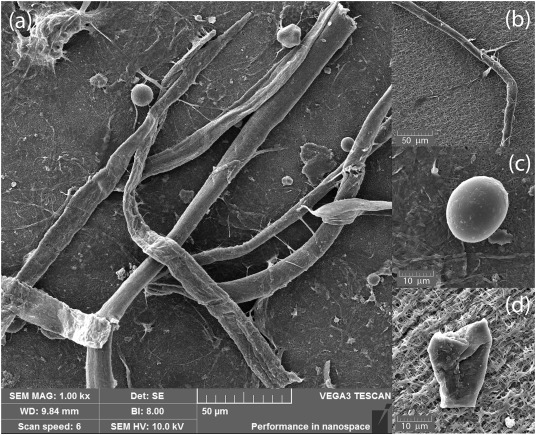
\includegraphics[width=0.5\textwidth]{electronico.jpg}
			\caption{Tamaño de partícula con microscopio electrónico}
			\label{electronico}
		\end{subfigure}
		\begin{subfigure}{0.45\textwidth}
		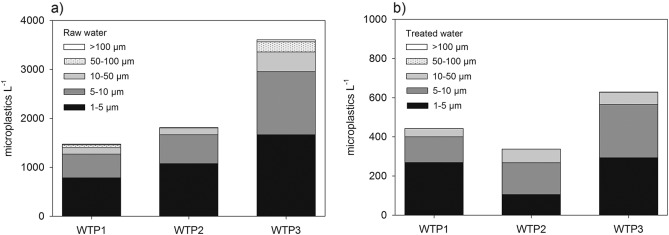
\includegraphics[width=1.2\textwidth]{size.jpg}
		\caption{Distribución de tamaño en agua libre y en agua tratada en las diferentes plantas de tratamientos}
		\label{size}
		\end{subfigure}
		
	\end{figure}
	
	\begin{figure}[H]
		\centering
		\begin{subfigure}{0.45\textwidth}
			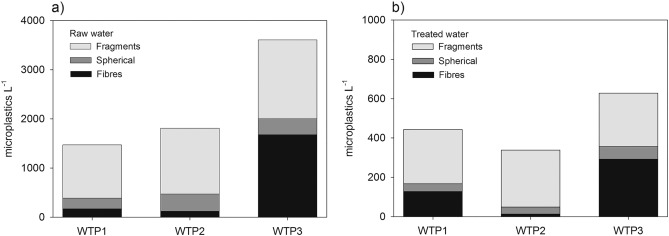
\includegraphics[width=1\textwidth]{proporcion.jpg}
			\caption{Proporciones de los diferentes MPs en agua sin tratar(a) y tratada(b)}
		\end{subfigure}
		\begin{subfigure}{0.45\textwidth}
			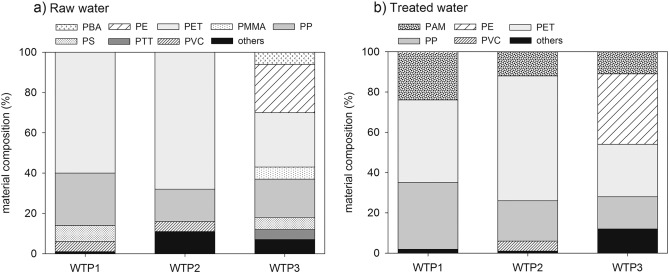
\includegraphics[width=1\textwidth]{composicion.jpg}
			\caption{Composición de de las partículas en agua sin tratar(a) y tratada(b)}
		\end{subfigure}
		
	\end{figure}
	\begin{figure}[h!]
		\centering
		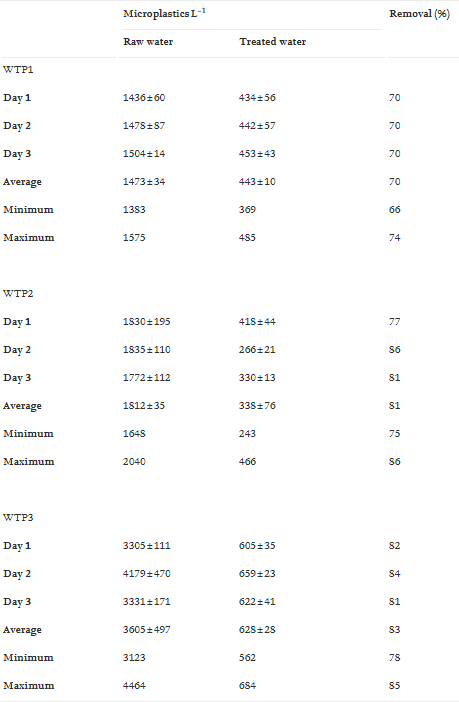
\includegraphics[scale=0.6]{tabla.png}
		\caption{Comparación de nuestros resultados con otros estudios}
	\end{figure}
	\begin{figure}[h]
		\centering
		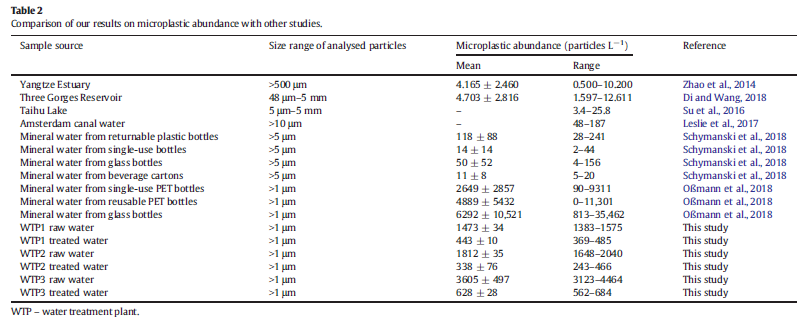
\includegraphics[scale=0.5]{tabla2.png}
		\caption{Comparativa de nuestros resultados con otros estudios}
		\label{tabla2}
		
	\end{figure}
	\begin{figure}[h]
	\centering
	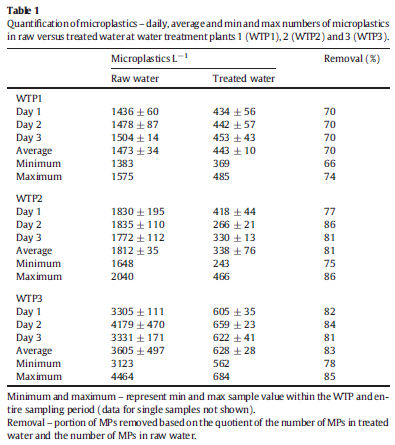
\includegraphics[scale=0.5]{tabla3.png}
	\caption{Comparativa de nuestros resultados con otros estudios}
	\label{tabla3}
	
	\end{figure}

\section{Fórmulas}
	Aunque todos los cálculos fueron realizados mediante computación con el programa R, aquí se recogen algunas de las fórmulas usadas:\\
	La varianza la denotamos por: $\sigma^2=\frac{\sum_{i=1}^{n}x_{i}^2*f_{i}}{\bar{X}}-(\bar{X}^2)$\\
	La ecuación de la recta: $y=mx+b$\\
	Al hacerse uso de la Inferencia estadística, tenemos:\\
	La media o esperanza: $\bar{x}=\frac{1}{n}\sum_{i=1}^{n}x_{i}$\\
	La cuasivarianza muestral:
	$S_{c}^{2}=\frac{1}{n-1}\sum_{i=1}^{n}(x_{i}-\bar{X})^{2}$\\
	Cuasivarianza tipica muestral:
	$S_{c}=\sqrt{S_{c}^{2}}$\\
	Intervalo de confianza para estimar $\mu$ ($\sigma^{2}$ conocida):
	$I_{(1-\alpha)}(\mu)=[\bar{X}-z_{\alpha/2}\frac{\sigma}{\sqrt{n}},\bar{X}+z_{\alpha/2}\frac{\sigma}{\sqrt{n}}]$\\
	Distribución binomial aproximada como una normal:
	$N(p,\sqrt{\frac{pq}{n}})$\\
	Intervalo de confianza para la proporción:
	$I=[p'-z_{\alpha/2}\sqrt{\frac{p'q'}{n}},p'+z_{\alpha/2}\sqrt{\frac{p'q'}{n}}]$\\
	Esperanza: $E=z_{\alpha/2}\frac{\sigma}{\sqrt{n}}$\\
	Tamaño de la muestra: $n=(z_{\alpha/2}\frac{\sigma}{E})^{2}$
	
	\bibliographystyle{plain}
	\bibliography{referencias}
\end{document}